\documentclass[a4paper]{article}
\usepackage{amsmath}
\usepackage{amsfonts}
\usepackage{amsthm}
\usepackage{amssymb}
\usepackage[english]{babel}
\usepackage{float}
\usepackage{graphicx}
\usepackage{hyperref}
\usepackage[utf8]{inputenc}
\usepackage{listings}
\usepackage{xcolor}
%% \usepackage{subfigure}
\usepackage{graphicx}
\usepackage{subcaption}
\usepackage{stmaryrd}

\usepackage{a4wide}
\usepackage{url}

\usepackage{appendix}

\graphicspath{{imgs/}} %Setting the graphicspath

\lstset{
  frame=tb,
  language=Python,
  aboveskip=3mm,
  belowskip=3mm,
  showstringspaces=false,
  formfeed=newpage,
  tabsize=4,
  comment=[l]{\#},
  breaklines=true,
  morekeywords={models, lambda, forms}
}

\newcommand{\prob}[1]{\mathbb{P}\left(#1\right)}
\newcommand{\expect}[1]{\mathbb{E}\left(#1\right)}
\newcommand{\bt}[1]{\mathbf{#1}}
\newcommand{\avg}[1]{\sum_{i=1}^{#1}X_i}
\newcommand*{\QEDA}{\hfill\ensuremath{\blacksquare}}%

\newcommand{\nt}{\text}
\newcommand{\lagr}{\mathcal{L}}
\newcommand{\isum}{\sum^\infty_}
\newcommand{\f}{$f$}

\title{\vspace{-5cm} Numerical Optimization \\ Re-exam Handin 4}
\author{Dmitry Serykh (qwl888)}

\begin{document}
\maketitle
\section{The Setup}
I implemented the Trust Region optimizer by following the basic algorithm
structure, outlined Algorithm 4.1 and then solved the Sub-problem 4.7 (finding
the value of $p$), such that the conditions from the Theorem 4.1 are satisfied
(4.8a, 4.8b and 4.8c).
%% \[
%% \begin{aligned}(B+\lambda I) p &=-g \\ \lambda\left(\Delta-\left\|p\right\|\right) &=0 \\(B+\lambda I) & \text { is positive semi-definite } \end{aligned}
%% \]

\subsection{Solution to the subproblem}
I decided to implement and experiment with both methods. I
validated the implementation by checking if all three conditions hold for the
found value of $\lambda^*$.
I determined experimentally that the first approach exhibits better performance
and the minima of the case function are found in fewer iterations, hence it was
chosen.

\subsubsection{Algorithm 4.3}
\label{subsubsec:43}
The first method, that I tried was from Section 4.3, and
Algorithm 4.3 in particular. It is based on root-finding Newton's Method and Cholesky
factorization that is used to iteratively find the values of $\lambda$.\\\\
I have added a safeguard, such that the Cholesky factorization always exists.
I set the initial value of $\lambda^{0}= -\lambda_1^e + c$, where $c$ is a small
constant and $\lambda_1^e$ is the smallest eigenvalue of $B$. This way, I make
sure that $\lambda^{(\ell)} > -\lambda_{1}$, and hence all eigenvalues of $(B + \lambda^{\ell}I)$
would be positive and indefinite Hessians would not cause any problems.\\\\
The book does not specify any stopping criterion for the Algorithm 4.3. I
decided to use a treshold parameter, such that the iteration would
terminate when  $\| \lambda^{\ell} - \lambda^{\ell + 1} \| < \varepsilon $,
where $\varepsilon$ is some small constant.dditionally, I have added a shortcut
that is described on page 85 in the book. If $B$ is positive-definite and $\|
B^{-1}g \| \leq \Delta$, the procedure can be terminated immediately with
$\lambda^*= 0$. It is then easy to solve for $p^*$.


\subsubsection{Bijection}
\label{subsubsec:bijection}
I start with the same value of $\lambda_0$ as in the previous method.
Then I iteratively find the value of $\lambda_1$, I start by increasing
$\lambda$ by $2^0 \cdot | \lambda_0$, then by $2^1 \cdot | \lambda_0$ and so on.
This continues until I find a value of $\lambda_1$, s.t.
$\| p(\lambda_1) \| <\Delta$. Afterwards, I execute the algorithm as specified
in the assignment text. The algorithm details and the reasoning behind some of
the desertions are described in Section \ref{sec:theory}. Finally, the procedure is
terminated when the interval size ($\lambda_0 - \lambda_1$) reaches some small
constant $\varepsilon$.

\subsection{The hard case}
I have implemented the method, described on p.88, in order to handle the hard
case. $\lambda$ would equal $-\lambda_1$, and I can find $p$ by first solving for $\tau$:
\[
p=\sum_{j: \lambda_{j} \neq \lambda_{1}} \frac{q_{j}^{T} g}{\lambda_{j}+\lambda}
q_{j} + z\sqrt{\Delta - \sum_{j: \lambda_{j} \neq \lambda_{1}}
  \frac{\left(q_{j}^{T} g\right)^{2}}{\left(\lambda_{j}+\lambda\right)^{2}}}
\]
However, I did not get to test my solution, since I could not detect the hard
case happening in any of the case functions.


\subsection{Parameters}
I used following parameter values in my implementation. Some values were taken
from the literature, while others were determined empirically.
\begin{itemize}
\item Initial trust region radius ($\Delta_0 = 1$)
\item Maximum trust region radius $\tilde{\Delta}=10^3$
\item Lower bound for the actual/predicted reduction ratio $\eta=0.2$
\item Initial coefficient $\lambda^{0}= -\lambda_1^e + 0.001$
\item Tolerance $\varepsilon = 10^{-7}$ on the gradient magnitude
\item Tolerance $\varepsilon_{\lambda} = 10^{-7}$ for the both
  the iterative solutions to the trust region sub-problem.
\end{itemize}

\subsection{Calculation of $\rho$}
The calculation of $\rho$ is an important part of the algorithm, and it is
calculated by:
\[
\rho_{k}=\frac{f\left(x_{k}\right)-f\left(x_{k}+p_{k}\right)}{m_{k}(0)-m_{k}\left(p_{k}\right)}
\]
However, I have experienced a problem with minimization of some functions.
The step was getting so small, that the denominator of the fraction above
was disappearing. Therefore, I have added a small constant (close to machine
precision) to the denominator to prevent this from happening.


\section{Testing protocol}
In order to test the effectiveness of my implementation, I came up with a
testing protocol, where I used following metrics:
\begin{itemize}
\item The convergence plots with the number of iteration on the x-scale and the
  Euclidean distance between the current value of $x$ and the
  optimum. The resulting plot can be seen on Figure \ref{plt1}.
\item The convergence plots with the gradient magnitude.
  The resulting plot can be seen on Figure \ref{plt2}. 
\item Plot for the median trust region as a function of number of iterations for
  the Log-Ellipsoid function can be seen on Figure \ref{plt3}. Trust region is
  monotonically non-increasing throughout the execution of the algorithm for the
  Log-Ellipsoid function. I have also experimented with other functions, and for
  the Rosenbrock function, there are regions for which the radius is increasing.
  However, the general trend is for the radius to be decreasing throughout the
  execution of the algorithms. Intuitively, this also makes sense, since we are
  taking smaller steps when approaching the optimum, because the curvature is
  less pronounced there.
\item \textbf{Accuracy}. The Euclidean distance to the optimum at the
  termination point. The results can be seen on Table \ref{table1}.
  The performance of my implementation of the trust
  region algorithm is compared to the performance of the line search methods
  from the previous assignment, namely Steepest Descent and Newton's Algorithm.
\item \textbf{Efficiency}. The number of steps until the gradient
  magnitude reaches $10^{-7}$. The results can be seen on Table \ref{table2}.
\end{itemize}
I used a random starting point taken from the uniform distribution in the
interval between $-10$ to $10$ and repeated each optimization 100 times for all
metrics and took the median. This was done to remove the influence of the
starting position from the results of the optimization. I used the median
to minimize the effect of the outliers. \\\\
As suggested, I have modified my implementation of the Log-Epsilon function and
excluded the first Attractive Region function from the experiments.

\begin{figure}[H]
    \centering
    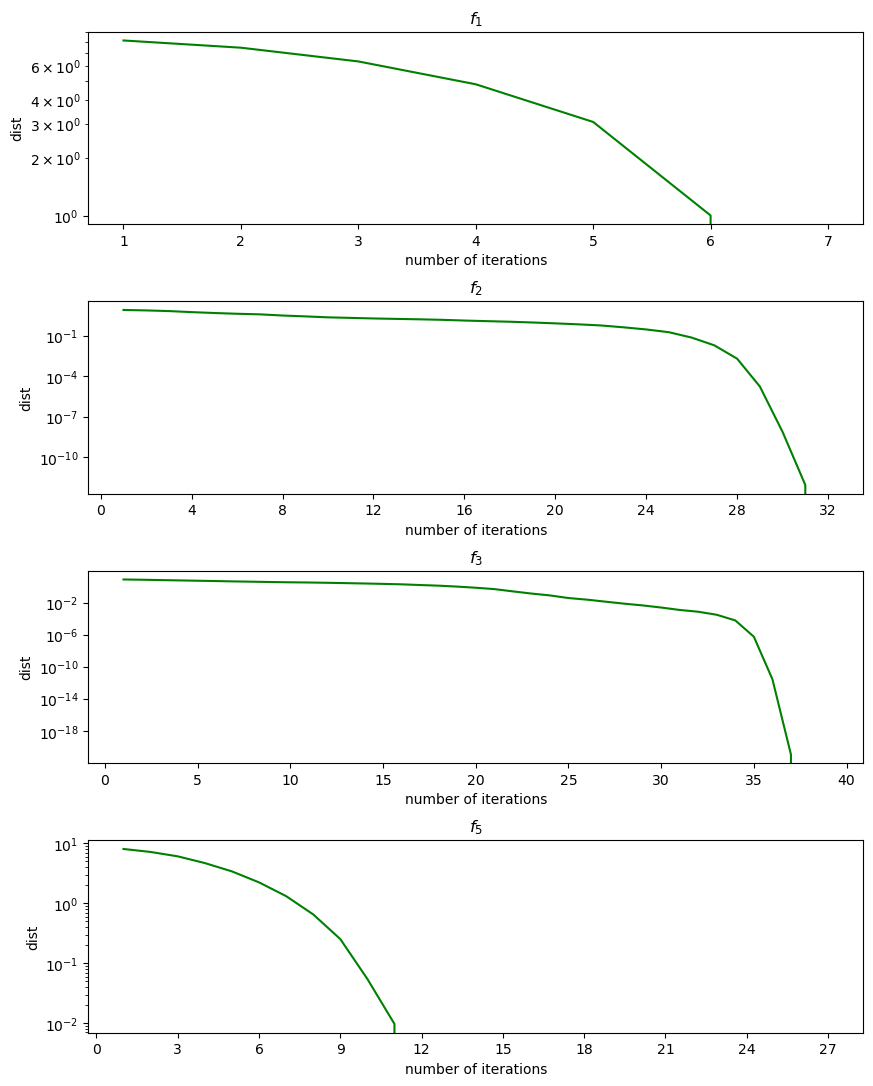
\includegraphics[width=0.7\textwidth]{plt_dist1000.png}
    \caption{Convergence plot of the median euclidean distance on the y-axis}
  \label{plt1}
\end{figure}

\begin{figure}[H]
    \centering
    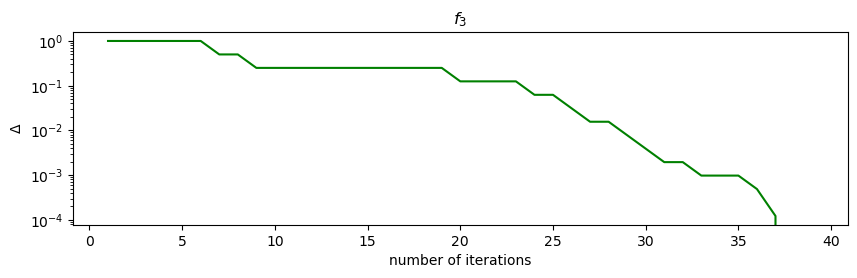
\includegraphics[width=0.7\textwidth]{plt_radius1000.png}
    \caption{Plot of the median trust region radius as a function of number of
      iterations for the Log-Ellipsoid function}
    \label{plt3}
\end{figure}

\begin{figure}[H]
    \centering
    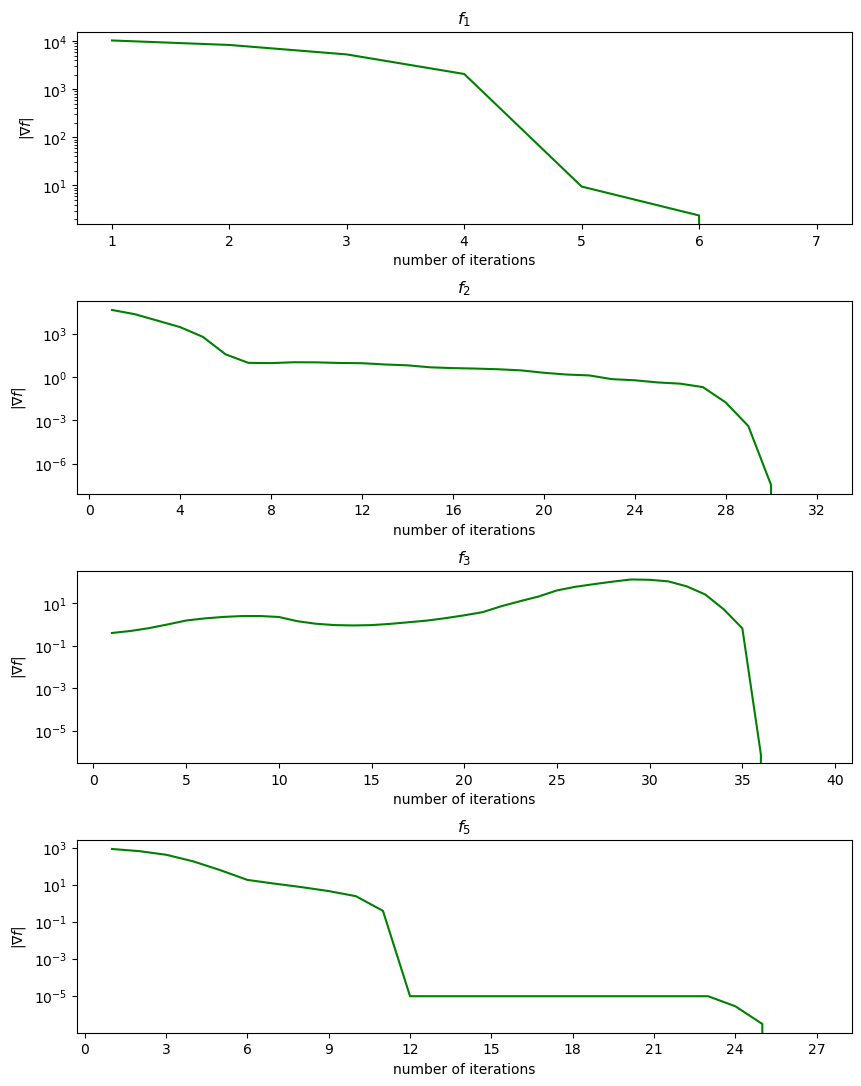
\includegraphics[width=0.65\textwidth]{plt_grad_norms1000.png}
    \caption{Convergence plot of the median gradient magnitude as a function of number of
      iterations}
  \label{plt2}
\end{figure}


\begin{table}[H]
\centering
\begin{tabular}{|l|l|l|l|l|l|}
\hline
                 & $f_1$         & $f_2$         & $f_3$       & $f_4$       & $f_5$       \\ \hline
stepest descent & $1.44\cdot10^{-4}$ & $7.59\cdot10^{-4}$ & $1.44\cdot10^{-10}$ & $6.51\cdot10^{-7}$ & $1.13\cdot 10^{-4}$ \\ \hline
newton           & $0.0$      & $8.15\cdot10^{-8}$ & $4.59\cdot10^{-16}$ & $6.4\cdot10^{-7}$  & $4.56\cdot10^{-7}$ \\ \hline
trust region    & $0.0$  & $1.05\cdot10^{-11}$ &  $1.72\cdot10^{-16}$ & n/a & $2.67 \cdot 10^{-7}$ \\ \hline
\end{tabular}
\caption{Average value of distance to the optimum at algorithm termination for 100 random starting points in the interval $[-10,10]$}
\label{table1}
\end{table}


\begin{table}[H]
\centering
\begin{tabular}{|l|l|l|l|l|l|}
\hline
                 & $f_1$  & $f_2$  & $f_3$   & $f_4$ & $f_5$  \\ \hline
stepest descent  & $3392$ & $6991$ & $5546$ & $488$ & $52$  \\ \hline
newton           & $1$    & $30$   & $16$   & $29$  & $2 $  \\ \hline
trust region     & $5$    & $32$   & $35$   & n/a   & $24 $ \\ \hline
\end{tabular}
\caption{Average number of iterations until algorithm termination for 100 random starting points in the interval $[-10,10]$}
\label{table2}
\end{table}

\section{Theoretical Part}
\label{sec:theory}
In the theoretical part, I choose the second option. \\\\
Problem 4.7 from the Book states:
\[
\min _{p \in \mathrm{R}^{n}} m(p)=f+g^{T} p+\frac{1}{2} p^{T} B p, \quad \text { s.t. }\|p\| \leq \Delta
\]
We assume that $B$ is strictly positive definite. I
will show that the described algorithm converges to $\lambda^*$, s.t
$p(\lambda^*) = p^*$\\\\
We know that $\| p(\lambda) \|$ is continuous and
strictly nonincreasing function in the interval $(-\lambda^e_1, \infty)$, where
$\lambda_1^e$ is the smallest eigenvector of $B$
(p.85 in the book). We then set $\lambda_0 = -\lambda^e_1$, since
$\lim_{\lambda \to -\lambda^e_1} \| p(\lambda) \| = \infty$
and find a value of $\lambda_1$, s.t. $\| p(\lambda_1) \| < \Delta$, which would
always exist, since we do not consider the hard case.
Hence for any $\lambda_a, \lambda_b, \lambda_c \in (-\lambda^e_1, \infty)$ s.t.
$\lambda_a \leq \lambda_b \leq \lambda_c$, we have that:

\[
\lambda_a \leq \lambda_b \leq \lambda_c \Leftrightarrow
\|p(\lambda_a)\| \leq \|p(\lambda_b)\| \leq \|p(\lambda_c)\| 
\]
Let $\lambda_n'$ be the value of $\lambda'$ at bisection iteration
$n \in \{0,1,2,...\}$, then:
\[
|\lambda_n' - \lambda^*| \leq
\left(\frac{1}{2}\right)^n (\lambda_0 + \lambda_1)
\]
and since:
\[
\lim_{n \to \infty} \left(\frac{1}{2}\right)^n = 0
\]
we have that:
\[
\lim_{n \to \infty} | \lambda_n' - \lambda^*| = 0 \Leftrightarrow
\lim_{n \to \infty} \lambda_n' = \lambda^*
\]
Hence, the algorithm would converge to $p(\lambda^*) = p^*$. Additionally, the
tolerance of this algorithm could be adjusted, since we have an
upper bound on the error and can use it to get the maximum number of iterations.\\\\
Regarding the indefinite case, I solve it by choosing the
$\lambda^{0}= -\lambda_1^e + c$, where $c$ is a small
constant and $\lambda_1^e$ is the smallest eigenvalue of $B$. This way, all the
eigenvalues would stay positive.

\section{Conclusion}
I have implemented the Trust Region algorithm, while experimenting with two
iterative solutions to the trust region sub-problem.
Algorithm manages to find the value of optimum of functions $f_1, f_2, f_3$ and
$f_5$ and its performance is much better than the Steepest Descent method, but
worse than the Newtons method that I have implemented in Assignment 3.

\end{document}


%% \section{Convergence Plots}
%% \label{sec:conv}
%% \begin{figure}[H]
%%   \centering
%%   \begin{subfigure}[b]{\textwidth}
%%     \centering
%%     \includegraphics[width=\textwidth]{plt_f_1.png}
%%     \caption{Ellipsoid Function}
%%   \end{subfigure}
%%   \begin{subfigure}[b]{\textwidth}
%%     \centering
%%     \includegraphics[width=\textwidth]{plt_f_2.png}
%%     \caption{Rosenbrock Function}
%%   \end{subfigure}
%%   \caption{Convergence Plots}
%%   \label{plt1}
%% \end{figure}
%% \end{document}
